%!TEX root = ../article.tex
\subsection{Individual View}
After observing an overview on data similarities, users may need to drill down to a few individual cases of interest for detailed examination.
We develop the Individual View for users to explore and compare the different individuals over time (\textbf{T6}).
% Specifically, our goal is to identify the important features at different time steps and their relationship to raw feature values (\textbf{T2}, \textbf{T4}).


\begin{figure}[t]
	\centering
    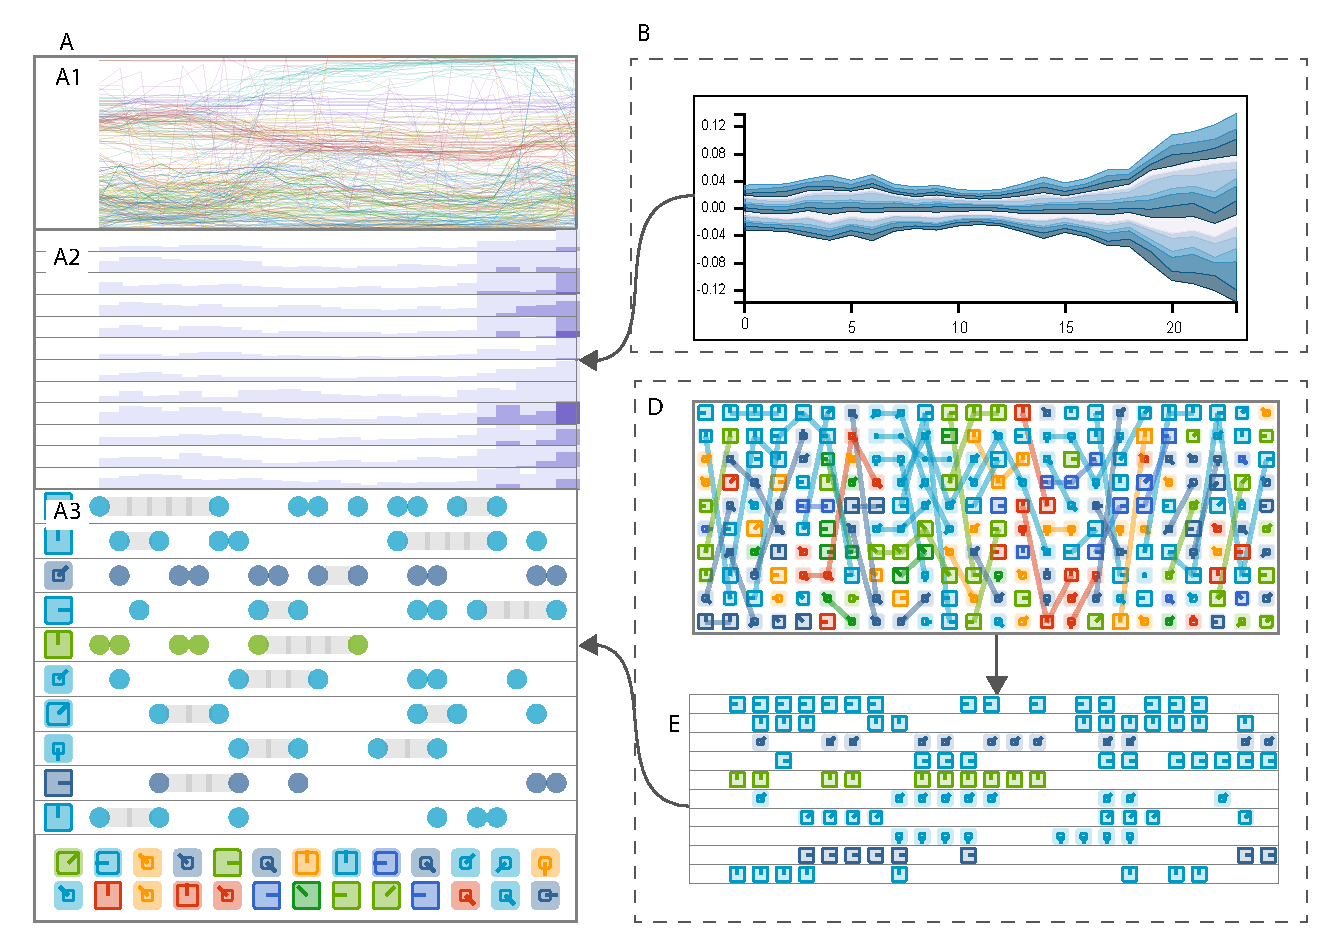
\includegraphics[width=0.90\textwidth]{figure/MultiRNNExplorer/design/alternative_design.pdf}
	\vspace{-3mm}
	\caption{Individual design and the alternative designs. A) Individual View. A1) Feature Trend Chart; A2) Cluster Importance Chart; A3) Top Features Chart. B) themeriver as the alternative design of the Cluster Importance Chart; C) and D) node-like sequence and node sequence as the alternative design of Top Features List.}
	\label{fig:individual_view}
	\vspace{-4mm}
\end{figure}

% cell -> card
\UC{The selected individual cases are visualized as several stacks of \UC{cell} as in Fig.~\ref{fig:individual_view}A.
Each cell consists of three components: the Feature Trend Chart (Fig.~\ref{fig:individual_view}A$_1$), the Cluster Importance Chart (Fig.~\ref{fig:individual_view}A$_2$), and the Top Feature List (Fig.~\ref{fig:individual_view}A$_3$).
All these three components share the same x-axis which represents the time where time steps increase from left to right.}

Feature Trend Chart is a multi-line chart that depicts how different features' values change over time. 
The y-axis represents normalized feature values where the feature value increases from bottom to top ranging between 0 and 1.
Each line represents a feature and the line color encodes feature category the same as in the Cluster View.
The corresponding lines are highlighted when hovering on any feature glyph in the Cluster View or hovering on feature importance view. 
% to enable users to focus on the features in the current context and avoid visual clutter.

The middle component is the Cluster Importance Chart, which is a list of horizon bar charts that summarize how each feature group's gradient changes over time.
Each feature group is represented as a \UC{horizon bar chart} and aligned vertically in the same order as the Cluster View.
For a horizon bar chart, each bar represents the averaged gradient for the corresponding feature group at one time step. 
We use both the bar height and bar color to encode the gradient value.
As shown in  Fig.\ref{fig:individual_view}A$_3$, the first visual channel to encode gradient value is bar height where a greater height indicates a larger gradient value.
When the gradient value exceeds a certain limit, we clip the bar and overlay another darker bar with the same height as the clipped part at the same position for better vertical space efficiency.
We have also considered other design choices such as a themeriver (Fig.\ref{fig:individual_view}B) in which each colored flow indicates a feature group. 
However, comparing different feature groups may be difficult and it requires more space when the gradient is large.
Thus, we abandon this alternative choice and adopt the current design.

\UC{
Though the Cluster Importance Chart provides an overview of how each feature cluster's importance changes over time, users still need to link this component to the Cluster View to observe which features are considered important by the model.
We design a Top Feature List to visualize the important features over time. 
Our first design is shown in Fig.~\ref{fig:individual_view}D. where the top $N$ features ranked by importance are visualized as feature glyphs at each timestamp. 
We draw links to connect glyphs that represent the same feature in consecutive time steps.
However, this design leads to serious visual clutter due to link overlap when feature ranks are frequently changed over time. 
To alleviate users' mental burden, we develop a new design as shown in Fig.~\ref{fig:individual_view}E.
% We visualize the top $N$ features that have the largest average gradients over time. 
Each feature is represented as a row and we draw its corresponding feature glyph at the timestamps when this feature is ranked in the top $N$ most important features. 
To simplify this visual design, we position the feature glyph at the beginning of each row. 
% As a feature has different gradients over time, the importance ranking of a feature can also vary at different steps.
We then use two colored circles linked with gray lines to indicate at which time steps the corresponding feature is ranked in the top $N$ mostly important features.
The circle color is consistent with the feature glyph color.
To make the Top Feature List space efficient, we only show ten rows by default, and other features are collapsed as feature glyph rows as shown in the bottom at Fig.\ref{fig:individual_view}A$_3$.
Users can click the glyph rows to select different features to analyze.
}

\UC{The three components enable users to observe which features are considered important by the model over time and how the importance is related to feature value changes.
Users can also append multiple cells to the Sequence View to compare different sequences side by side. 
When the number of cells becomes large, we use dbscan to cluster the similar individual cases by the fatten cluster importance(discussed in sec. \ref{section:feature_importance}) into one stacked cells with one randomly selected case as the representative case at the top of stack.}
